\begin{center}
\Huge
Funktionstyper 
\end{center}
\section*{Sammensatte funktioner}
\stepcounter{section}
En sammensat funktion er - som navnet hentyder til - funktioner, der er sat sammen. Mere præcist har vi en definition.
\begin{defn}
Har vi to funktioner $f$ og $g$, så kan vi bestemme  den sammensatte funktion af $f$ og $g$ som
\begin{align*}
f(g(x)).
\end{align*}
Dette skrives også til tider $f(g(x))= g\circ f(x)$. I dette tilfælde kaldes $g$ for den indre funktion og $f$ for den ydre funktion.
\end{defn}
\begin{exa}
Lad $f$ og $g$ være givet ved henholdsvist
\begin{align*}
f(x) = \sqrt{x} \textnormal{ og }g(x) = 3\cdot x.
\end{align*}
Så er den sammensatte funktion $f(g(x))$ bestemt ved
\begin{align*}
f(g(x)) = \sqrt{3\cdot x}.
\end{align*}
Tilsvarende er den sammensatte funktion $g(f(x))$ bestemt ved
\begin{align*}
g(f(x)) = 3\sqrt{x}.
\end{align*}
\end{exa}
\begin{exa}
CO$_2$-koncentrationen i en beholder kan tilnærmes ved $f(x) = 10\cdot x+385$, hvor $f$ er i ppm (parts per million) og $x$ er antallet af en bestemt type bakterier i mio. Antallet af bakterier (i mio.) i beholderen kan i et begrænset tidsinterval beskrives ved $g(t)= 2\cdot 1.07^t$, hvor $t$ beskriver tiden i timer. CO$_2$-koncentrationen som funktion af tid kan derfor beskrives ved
\begin{align*}
f(g(t)) = 10\cdot (2\cdot 1.07^t) + 385 = 20\cdot 1.07^t + 385.
\end{align*}
\section*{Stykvist definerede funktioner}
\stepcounter{section}
En stykvist defineret funktion er en funktion, der er defineret på forskellige måder alt efter hvad $x$ er.
\begin{exa}
Et taxafirma tager følgende pris for taxakørsel: De første to kilometer koster 10kr pr kilometer, de næste 5km koster 7 kr pr kilometer, og resten at afstanden koster taxaen 5kr pr kilometer. Vi kan definere prisen $p(x)$ som en stykvist defineret funktion:
\begin{align*}
p(x)=
\begin{cases}
10\cdot x, \ &0\leq x \leq 2,\\
7\cdot x + 6,\ &2 < x \leq 7,\\
5 \cdot x + 20,\ &7<x,
\end{cases}
\end{align*}
hvor $x$ er antal kilometer kørt og $p(x)$ er prisen i kr. 
\end{exa}
Grafen for $p$ kan ses på Fig. \ref{fig:stykvis}
\begin{figure}[H]
\centering
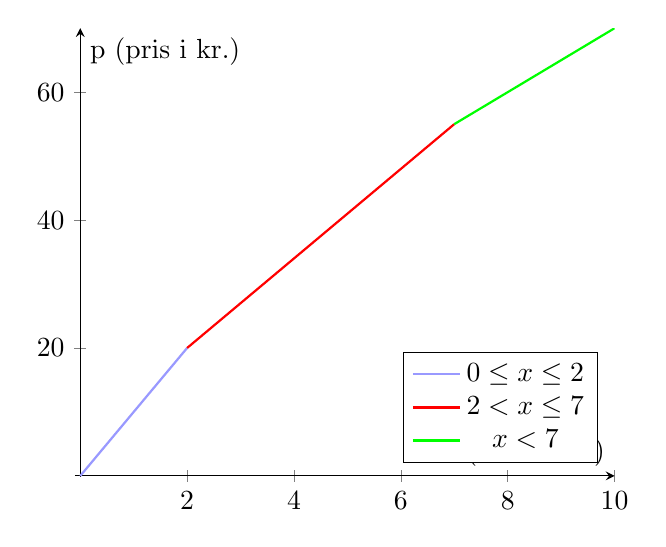
\begin{tikzpicture}
\begin{axis}[axis lines=middle, xmin = -0.1,ymin=-0.1,
legend pos = south east, 
xlabel={x (kørte km.)},
ylabel = {p (pris i kr.)}
]
\addplot[color=blue!40,samples = 1000, thick, domain = 0:2] {10*x};
\addplot[color=red,samples = 1000,thick,domain=2:7] {7*x+6};
\addplot[color=green,samples = 1000,thick,domain=7:10] {5*x+20};
\legend{$0\leq x \leq 2$,$2<x\leq 7$,$x<7$}
\end{axis}
\end{tikzpicture}
\caption{Pris for taxa som funktion af kørte km.}
\label{fig:stykvis}
\end{figure}
\end{exa}
\subsection*{Opgave 1}
For følgende funktioner $f$ og $g$, bestem så den sammensatte funktion $f(g(x))$ og $g(f(g))$.
\begin{align*}
&f(x) = \sqrt{x}\  \textnormal{ og } g(x) = x^2\\
&f(x) = 2x^3\  \textnormal{ og } g(x) = 10x+3\\
&f(x) = \ln(x)\  \textnormal{ og } g(x) = \frac{1}{x}\\
&f(x) = \sqrt[10]{x}\  \textnormal{ og } g(x) = x^{20}
\end{align*}
\subsection*{Opgave 2}
For $f(x) = x^2$ og $g(x)=2x+3$ løs ligningen
\begin{align*}
f(g(x)) = 0.
\end{align*}

\subsection*{Opgave 3}
Bestem for følgende funktion den indre og ydre funktion
\begin{align*}
	&1) \ \sqrt{2x+1}   &&2) \  2^{x^2-7}     \\
	&3) \ \frac{1}{-4x+12}   &&4) \ e^{2x-4}      \\
	&5) \ \ln(2x)   &&6) \  \log_5(7x^2)     \\
	&7) \ (x+10)^3   &&8) \  3^{\log_{10}(2x)+7}       \\
\end{align*}


\subsection*{Opgave 4}
En stykvist defineret funktion $f$ er givet ved
\begin{align*}
	f(x) = 
	\begin{cases}
		x^2, \ &\textnormal{ hvis } x > \geq 0,\\
		-x^2, \ &\textnormal{ hvis } x < 0.
	\end{cases}
\end{align*}
\begin{enumerate}[label=\roman*)]
	\item Bestem $f(3).$
	\item Bestem $f(-4).$
	\item Løs ligningen $f(x) = -64$.
\end{enumerate}

\subsection*{Opgave 5}
Prisen for at rejse $x$ kilometer med taxafirmaet taxA kan beskrives ved funktionen $f$ givet ved
\begin{align*}
	f(x) =
	\begin{cases}
		20x + 50, \ &\textnormal{ hvis } x \leq 8, \\
		16x + 82, \ &\textnormal{ hvis } 8 < x \leq 15, \\
		12x + 142, \ &\textnormal{ hvis } 15 < x.
	\end{cases}
\end{align*}

\begin{enumerate}[label = \roman*)]
	\item Bestem prisen for at køre 10km med taxA.
	\item Afgør, hvor langt man kan køre for 250 kr.
	\item Tegn grafen for $f$ i Maple og verificér dit svar fra i) og ii).
\end{enumerate}

